\documentclass[biblatexieee]{kclthesis}

\title{Argument Mining on Social Media}
\author{Danielius Marciukovas}
\modulecode{7CCSMPRJ}
\department{Department of Informatics}
\submissiontitle{Individual Project Submission 2018/19}
\studentnumber{1844311}
\emailaddress{danielius.marciukovas@kcl.ac.uk}
\programme{MSc Web Intelligence}
\supervisor{Josh Murphy}
\wordcount{14927}

\makenomenclature
\makeglossaries

\begin{document}
    \pagenumbering{gobble}
    
    \maketitle
    % \newpage
% \thispagestyle{empty}
% \mbox{}
% \newpage
    \section*{Abstract}
Lorem ipsum dolor sit amet, consetetur sadipscing elitr, sed diam nonumy eirmod tempor invidunt ut labore et dolore magna aliquyam erat, sed diam voluptua. At vero eos et accusam et justo duo dolores et ea rebum. Stet clita kasd gubergren, no sea takimata sanctus est Lorem ipsum dolor sit amet. Lorem ipsum dolor sit amet, consetetur sadipscing elitr, sed diam nonumy eirmod tempor invidunt ut labore et dolore magna aliquyam erat, sed diam voluptua. At vero eos et accusam et justo duo dolores et ea rebum. Stet clita kasd gubergren, no sea takimata sanctus est Lorem ipsum dolor sit amet. 
    \mbox{}\newline\vspace{10mm} \mbox{}\LARGE
%
{\bf Acknowledgements} \normalsize \vspace{5mm}

I would like to thank my supervisor for providing me valuable support and feedback all throughout the year since I met him. He was helpful in guiding me in the right direction when I needed it and able to provide clearance on any matter whenever I had any concerns or questions. 

    \pagenumbering{roman}
\setcounter{tocdepth}{4}
\tableofcontents
\newpage
    \newpage

\newacronym{ai}{AI}{Artificial Intelligence}
\newacronym{nlp}{NLP}{Natural Language Processing}
\newacronym{ml}{ML}{Machine Learning}
\newacronym{te}{TE}{Textual Entailment}
\newacronym{af}{AF}{Argumentation Framework}
\newacronym{aaf}{AAF}{Abstract Argumentation Framework}
\newacronym{baf}{BAF}{Bipolar Argumentation Framework}
\newacronym{am}{AM}{Argumentation Mining}
\newacronym{edits}{EDITS}{Edit Distance Textual Entailment Suite}
\newacronym{api}{API}{Application Programming Interface}
\newacronym{eop}{EOP}{Excitement Open Platform}
\newacronym{rnn}{RNN}{Recurrent Neural Network}
\newacronym{lstm}{LSTM}{Long Short-Term Memory}
\newacronym{snli}{SNLI}{Stanford Natural Language Inference}
\newacronym{ram}{RAM}{Rapid-Access Memory}
\newacronym{cpu}{CPU}{Central Processing Unit}
\newacronym{gpu}{GPU}{Graphics Processing Unit}
\newacronym{vram}{VRAM}{Video Rapid-Access Memory}
\newacronym{csv}{CSV}{Comma-Separated Values}
\newacronym{os}{OS}{Operating System}
\newacronym{glove}{GloVe}{Global Vectors for Word Representation}
\newacronym{ddos}{DDoS}{Distributed Denial of Service}
\newacronym{url}{URL}{Uniform Resource Locator}
%\newglossaryentry{pi}{name={\ensuremath{\pi}}, description={ratio of circumference of circle to its diameter}, sort=pi}
%\newglossaryentry{Linux}{name=Linux,description={is a generic term referring to the family of Unix-like computer operating systems that use the Linux kernel}, plural=Linuces}
\printglossaries

\newpage
    \thispagestyle{empty}
\listoffigures
\listoftables
\lstlistoflistings
\newpage
    \fancyhead{}
    \fancyfoot{}
    \pagestyle{fancy} 
    \fancyhead[R,L]{\sffamily\small \thepage}
    \fancyhead[LO]{\sffamily\small \nouppercase{\rightmark}}
    \renewcommand{\headrulewidth}{0.4pt}
    \renewcommand{\footrulewidth}{0.0pt}
    
    \pagenumbering{arabic}
    \section{Introduction}
\subsection{Overview} 
 Argumentation is a subject that studies processes involved in reasoning and the structure of reason itself. It is a field that encompasses and spans across multiple other fields, most notably language, philosophy, psychology, logic and has recently transcended into \gls{ai}. This is because \gls{ai} provides the ability to conjoin mental reasoning models and mathematical models for automated reasoning \citep{Lippi2016ArgumentationMS}. The applications of argument models within computer science and \gls{ai} are vast in possibilities. The ability to view and model such arguments provides important insight into how humans reason about different claims, how the claims are supported or disagreed with. Given an argument model applied to a discussion forum or a debate, this would provide an opportunity to understand more deeply and extract points of view that carry the most weight \citep{Cocarascu2017MiningBA}. Subsequently, it would be possible to analyse the flow of the discussion and see how the positions taken within the debate change over time as new arguments are introduced. On the other hand, same argument models can also allow us to investigate how a certain perception of something (review, feedback, etc.) can be altered \citep{ApproxToTruth}. Also, this is a hot topic with regards to ethics within the \gls{ai} system. The decisions that we delegate to \gls{ai} to make, have to be verifiable, thus meaning the system has to be able to show the arguments that it worked with and how the consensus on the decision was made. All in all, industries that would benefit would be law, politics and political debates, reviews and marketing, social media platforms to name a few.
 
\subsection{Argument Mining}
 
 \gls{am} is an intensive research field focused on automatically extracting arguments and their interrelationships from text documents. Due to recent technological advancements in other fields such as \gls{ai}, \gls{nlp} and \gls{ml}, this is becoming more and more possible. Moreover, internet provides unlimited amounts of data to analyse and extract arguments from with accessibility to websites such as Facebook, Twitter, Wikipedia Talks, Reddit and other popular social media pages 
 
 Unfortunately, this is not easy to do. The definition of argument is hard to express in mathematical or computer science terms. First of all, there are no limits as to how long an argument should be. An argument, depending on the corpora, can be a part of a sentence or the whole document could be one big argument backed by many smaller arguments within it (e.g. a certain law article is broken down into sections, which are then broken down into paragraphs and so on). Secondly, the nature of the argument has to be understood, to determine whether it is supporting any other argument, or attacking it. An argument is considered to be a supporting argument if it is on point with the view made by the previous original argument. Conversely, going back to the law example, an attack to the argument could be considered in the sense of an exception that is stated within the law, where the law doesn't apply. 
 
 These points coupled together mean that argument classification problem is dependent on meaning of the argument itself, which makes this also a \gls{nlp} problem. Context or topic of the corpora matters a lot as well, because of language stylistic differences. It is no surprise that legal documents entail a more precise syntactical text structure, due to the nature of the industry requiring concrete descriptions to cover and exclude very specific cases of application. On the other hand, texts found in social media are of a more diverse linguistic composition, where messages posted by users can be very conversational or carry a meaning that is only understood by a certain group of people (e.g. abbreviations, specific background required).

\subsection{Project Aims and Objectives} 
 The aim of this project is to gain an up to date knowledge of current trends and advancements within the field of argumentation mining, to create a tool that given a specific chain of arguments in text form would analyse such arguments and construct an \gls{af} displaying the winning or most convincing arguments, and to contribute to the research community by explaining views and sharing ideas pertaining to the problem at hand.

\subsection{Background and Literature Survey} \label{sub:background}

This part is for literature review.

% It gives an overall picture about the work with a clear review of the relevant literature.  The background of the project should be given.  What have been done to deal with the problem should be stated clearly.  The pros and cons of various existing algorithms and approaches should be stated as well.  Differences between your proposed method and the existing ones should be briefly described. 

%The following links may help on the literature review: IEEE Xplore digital library: a resource for accessing IEEE published scientific and technical publications. (You must be with King's network to get access to the digital library) ScienceDirect.com: an electronic database offering journal papers not published by IEEE (You must be with King's network to get access to the database)

    \section{Background Theories} 

This section describes what the reader has to know in order to understand my project.
    \section{Literature Review}
    \subsection{Overview}
        In \autocite{Lippi2016ArgumentationMS}, the authors focus on giving the reader a broad overview of argumentation and various computational challenges associated with it. Authors proceed to entertain the thoughts of what the breakthrough by solving these challenges would mean on a societal level and the impact of it. Moving on, the paper also describes different approaches that were previously experimented within the domains of argumentation and \gls{am}, mainly extracting arguments from unstructured text, which authors consider to be the core \gls{am} task. The core \gls{am} tasks are explained sufficiently for the reader to understand the differences between them. On the other hand, authors give only brief mentions to other \gls{am} tasks (opinionated claim analysis, premise verification, etc.), without giving a clear description of how they are different from each other. Also, the article does not provide any concrete evaluation of each methods, which makes it hard to gauge which approach has been the most successful so far or what the results were. Overall, the authors give a good overview of active research topics and different directions that the domain has taken.
        
    \subsection{Textual Entailment}
        \gls{te} is one of the most popular approaches to identify argument \textit{attack} and \textit{support} relationships. The \autocite{Cabrio2012NaturalLA, Cabrio2012CombiningTE} papers give a general introduction to using \gls{te} as a means for identifying how one argument stands in relation to the other. Authors make a strong assumption that \textit{support} relation in \gls{baf} is the same as \textit{entailment} in \gls{te} and \textit{attack} in \gls{baf} is as \textit{contradiction} in \gls{te}. They test this theory on a set of arguments gathered from Debatepedia, an online debate forum where users express pros and cons on various topics. The language used at such discussions is quite different from loose and unstructured linguistics that can be seen in online social media corpus, which makes it hard to predict how the approach would do given a unpredictable environment. The system used for deciding if there exists a relation is called \gls{edits}, which states that the entailment relation probability of two arguments in a pair is greater the lower the number of changes need to be made between those two arguments, and vice versa. The chosen argument pair set is small, only 200 (100 used as a training set and 100 as test set), which is arguably insufficient to accurately assess the proposed approach, nevertheless, authors managed to accurately compute argument interrelations 75\% of the time, which is better than expected. In \autocite{Cabrio2013ANL, Cabrio2013DetectingBS}, the same authors have improved upon their research by exploring the \textit{support}-\textit{entailment} relationship, mostly by taking a step back on their previous assumption. The authors give an overview of semantic inferences in \gls{nlp}, in the sense that it is not always the case that an argument that supports another argument necessarily entails the latter argument in context. This was done by introducing a third labelling of argument pairs as \textit{null}, when such relation cannot be determined just from looking at those two arguments. Subsequently, same approach was applied to attacks, mainly by introducing 4 different types of complex attacks (\textit{supported}, \textit{mediated}, \textit{secondary}, \textit{extended}). The idea is similar, in that not all \textit{attacks} are \textit{contradictions}, thus making this case more subtle in general, requiring additional specification to identify attack relations. The results show that approximately 60\% of support argument pairs - \gls{te} holds; and for attacks - contradiction is present in about 70\% of argument pairs.
     
        Recently, the research in \gls{am} has taken a turn to social media, namely Twitter. Twitter is different from Debatepedia in that it often contains noisy, unstructured messages. This is mostly because of the specific restriction that Twitter imposes, being 140 character limit, which forces the user to express thoughts in short. Twitter is a good choice, because it provides open \gls{api} and it is possible to filter messages based on specific topics, that are defined with the use of a hashtag symbol (\#). In \autocite{Bosc2016DARTAD}, the authors describe their methodology for classifying tweets as argumentative or non-argumentative. The methodology provides extensive description of how to treat different types of tweets, how to evaluate the substance of each tweet and shows relevant examples. A further study \autocite{Bosc2016TweetiesSP} by the same authors put such dataset to practice. The paper divides the work into 4 major steps that have to be taken from start to finish and discusses different approaches within each of those steps. The steps are as follows: \textit{1)} tweets need to be separated into two pools - either argumentative or non-argumentative; \textit{2)} argumentative tweets need to be further divided into separate groups by topic, and then, argument pairs have to be created; \textit{3)} argument relationship within the argument pairs have to be predicted as either \textit{attack} or \textit{support}; \textit{4)} argumentation graph has to be built. First and second tasks are trivial compared to the third one, as is evident based on views expressed in the paper. Different approaches were tested while tackling the third task, \gls{eop}, \gls{te}, neural sequence classifiers, though all with unsatisfying results, accuracies being less than 20\%.
     
    \subsection{Other Approaches}
        Here are briefly described other methods that were taken to extract arguments from unstructured texts:
        \begin{itemize}
            \item The \autocite{Cocarascu2017IdentifyingAA} paper uses Deep Learning and Long-Short Term Memory unidirectional and bidirectional networks to classify relations as either \textit{attack}, \textit{support} or \textit{neither support nor attack} and achieved an accuracy of 89.53\%. 
            
            \item In \autocite{Cocarascu2017MiningBA} the authors employ a methodology that tries to discover argument relations by grouping arguments into groups of similar topics. They showcase this by using an example containing hotel reviews, with reviews being grouped into 6 different topics. Also, the paper gives a brief description of how each topic could be given a strength score based on existing arguments.
            
            \item The \autocite{ApproxToTruth} paper analyses how a part of online comment network relates to the whole network in terms of acceptable conclusions drawn. In other words, by reading through an online debate, how similar conclusions can be drawn at that point in time compared to the overall consensus of the debate taking into equation all existing arguments. This is done by comparing grounded extensions of the two argumentation frameworks.
            
            \item The \autocite{Cocarascu2016DetectingDR} gives a \gls{ml} approach to detecting deceptive reviews by constructing topic independent \gls{aaf} and topic dependent \gls{baf}. Several algorithms (Random Forests, Logistic Regression, Na{\"i}ve Bayes) are used to evaluate the performances.
            
            \item In \autocite{Dusmanu2017ArgumentMO} supervised classification algorithms are used to detect arguments on Twitter. Authors also propose new avenues for research, namely facts recognition and source identification with regards to arguments.
            
            \item In \autocite{Lippi2015ContextIndependentCD}, the authors provide a context independent (topic independent) methodology for automatically extracting argument frameworks from unstructured text. They do this by splitting text into sentences and for each sentence building tree structures representing syntactical components of a sentence. The results are quite satisfactory with 74.6\%/68.4\% of precision/recall performances.
        \end{itemize}
    \section{Professional Issues and Ethical Considerations}
    
    \newcolumntype{L}{>{\centering\arraybackslash}m{5cm}}
\newcolumntype{S}{>{\centering\arraybackslash}m{35mm}}
\newcommand\setrow[1]{\gdef\rowmac{#1}#1\ignorespaces}
            
\section{Requirements Specification}
    \subsection{Product Functions}
        This section discusses the software requirements and explains the rationale behind them.
        Firstly, \autoref{table:coreproductfunc} presents core functions that the software has to be able to perform. Each of the core functionalities are explained in more detail later on.
        
        \begin{table}[!htbp]
            \centering
            \caption{Core Product Functions}
            \begin{tabular}{|>{\bfseries}c|L|c|}
                \toprule
                \textbf{Function} & \textbf{Description} & \textbf{Priority Level} \\ 
                \midrule 
                1 & Download LSTM Data Sets & Medium \\ \hline 
                2 & Data Mine Tweets & High \\ \hline 
                3 & Develop \gls{lstm} Neural Network & High \\ \hline 
                4 & Build a Graph Representation of LSTM Predictions & High \\ \hline  
                5 & Perform \gls{baf} Analysis & High \\ 
                \bottomrule
            \end{tabular}
            \label{table:coreproductfunc}
        \end{table}
        
        Each function has a priority level attached to it. High priority represents a necessity, a functionality that is expected to be a part of the minimum viable product. Medium priority describes a case where the functionality is not critical, but provides a useful addition to overall performance of the software. Low priority is generally a nice-to-have, focusing on ease of software use, intermittent result saving for additional future analysis or user experience, e.g. informing the user of currently performed actions or steps.
        
        \subsubsection{LSTM Data Download Requirements}
            Requirements for Automating the download of required data either for processing or \gls{lstm} training are described here (\autoref{table:func1spec}.
            
            \begin{table}[!htbp]
                \centering
                \caption{Function 1 Specifics}
                \begin{tabular}{|>{\bfseries}c|L|c|}
                    \toprule
                    \textbf{Function} & \textbf{Description} & \textbf{Priority Level} \\ 
                    \midrule 
                    1.1 & Download GloVe Vector Data & High \\ \hline 
                    1.2 & Download \gls{snli} Data & Low \\ \hline 
                    1.3 & Extract/Unzip Downloaded Data & Medium \\
                    \bottomrule
                \end{tabular}
                \label{table:func1spec}
            \end{table}
            
            \gls{glove} data is on high priority because it describes how sentences consisting of words and characters are to be transformed into numerical multidimensional arrays for \gls{lstm} processing. This is required for use with Twitter data and \gls{lstm} training, validation and testing purposes as well.
            
            On the other hand, \gls{snli} data is only used for training and testing of \gls{lstm}. Because training of the model is done beforehand, the user would not need to worry about this unless the goal is to train a different \gls{lstm} model (and use it).
            
        \subsubsection{Twitter Data Mining Requirements}
            Specific functional requirements for Data Mining on Twitter are presented here. The \autoref{table:func2spec} lists what is meant by "Data Mining" and what processes it involves.
            
            \begin{table}[!h]
                \centering
                \caption{Function 2 Specifics}
                \begin{tabular}{|>{\bfseries}c|L|c|}
                    \toprule
                    \textbf{Function} & \textbf{Description} & \textbf{Priority Level} \\ 
                    \midrule 
                    2.1 & Input Search Term or Topic to Mine & High \\ \hline 
                    2.2 & Save Data Mined Tweets into .csv File & Medium \\ \hline 
                    2.3 & Remove Non-Alphanumerical Characters & High\\ \hline
                    2.4 & Remove Stop Words & High \\ \hline
                    2.5 & Lemmatize words & High \\ \hline
                    2.6 & Remove Duplicate Tweets & High \\ \hline
                    2.7 & Filter Short Tweets & Low \\ \hline
                    2.8 & Read Tweets from Saved .csv File & Medium \\
                    \bottomrule
                \end{tabular}
                \label{table:func2spec}
            \end{table}
            
            The requirements here are mostly concerned with cleaning the mined data. This involves removal of non-alphanumerical characters, such as twitter hashtags (\#), links to other websites, mentions of other users (\@), as well as the removal of stop words, duplicate or too short (e.g. single word) tweets, performing lemmatization.
        
        \subsubsection{LSTM Development Requirements}
            \gls{lstm} is the core of this software, because it serves the most important task of accurately predicting argument relations and directions, thus all of its' functional requirements are in high priority.
            
            \begin{table}[!htbp]
                \centering
                \caption{Function 3 Specifics}
                \begin{tabular}{|>{\bfseries}c|L|c|}
                    \toprule
                    \textbf{Function} & \textbf{Description} & \textbf{Priority Level} \\ 
                    \midrule
                    3.1 & Process \gls{glove} Vector Data & High \\ \hline
                    3.2 & Perform \gls{lstm} Training & High \\ \hline
                    3.3 & Perform \gls{lstm} Validation & High \\ \hline
                    3.4 & Perform \gls{lstm} Testing & High \\ \hline
                    3.5 & Perform \gls{lstm} Prediction on Tweets & High \\ \hline
                    3.6 & Perform With 75\% Accuracy Or More & High \\ \hline
                    3.7 & Save Successfully Trained \gls{lstm} Model & High \\ \hline
                    3.8 & Load Existing Specified \gls{lstm} Model & High \\
                    \bottomrule
                \end{tabular}
                \label{table:func3spec}
            \end{table}
        
        \subsubsection{Graph Network Requirements}
            The Graph is one of the main ways to represent argument frameworks and analyse them. The requirements are listed in \autoref{table:func4spec}.
            
            \begin{table}[!htbp]
                \centering
                \caption{Function 4 Specifics}
                \begin{tabular}{|>{\bfseries}c|L|c|}
                    \toprule
                    \textbf{Function} & \textbf{Description} & \textbf{Priority Level} \\ 
                    \midrule
                    4.1 & Create a Node for Each Argument Mined & High \\ \hline
                    4.2 & Create an Edge for Each Argument Relation & High \\ \hline
                    4.3 & Differentiate Attack and Support Edges & High \\ \hline
                    4.4 & Save Graph Data into .gexf File & Low \\ \hline
                    4.5 & Load Graph Data from .gexf File & Low \\ \hline
                    4.5 & Display Computed Directed Graph & Medium \\
                    \bottomrule
                \end{tabular}
                \label{table:func4spec}
            \end{table}
            
            Each vertex represents an argument, and an edge - relation between those arguments. The resulting graph must be Digraph, with different edges for \textit{attack} and \textit{support} relations.
        
        \subsubsection{Argument Framework Analysis Requirements}
            The requirements for \gls{af} analysis state steps that need to be taken in order to compute the grounded extensions of argument graphs.
            
            \begin{table}[!htbp]
                \centering
                \caption{Function 5 Specifics}
                \begin{tabular}{|>{\bfseries}c|L|c|}
                    \toprule
                    \textbf{Function} & \textbf{Description} & \textbf{Priority Level} \\ 
                    \midrule 
                    5.1 & Compute Conflict Free Arguments & High \\ \hline 
                    5.2 & Compute Admissible Arguments & High \\ \hline 
                    5.3 & Compute the Grounded Extension Arguments & High \\ \hline 
                    5.4 & Print to Console the Grounded Extension & Medium \\
                    \bottomrule
                \end{tabular}
                \label{table:func5spec}
            \end{table}
            
            This part of software is also very important, because argument frameworks are what is used to analyze argumentation in \gls{ai}. Thus, high priority levels for each computational requirement listed in \autoref{table:func5spec} are in line with the goal of the project.
        
    \subsection{Operating Environment}
        This section describes the hardware and system requirements that the software must be able to run on. These requirements are important because not every hardware is going to be able to handle the same amounts of data or in the same amount of time. 
        
        \begin{table}[!htbp]
            \centering
            \caption{Operating Environment}
            \begin{tabular}{|>{\bfseries}S|L|S|}
                \toprule
                \textbf{Hardware/System} & \textbf{Description} & \textbf{Value} \\ 
                \midrule
                \gls{cpu} & Responsible for running applications and performing calculations & Intel i7-7700 \@4.2GHz\\ \hline
                \gls{ram} & Responsible for storing data that is currently in use by the \gls{cpu} & 16.0GB\\ \hline
                \gls{gpu} & Draws graphics. \gls{lstm} component of this software is run on this part as well & nVidia 1080Ti GTX \\ \hline
                \gls{vram} & Same as \gls{ram}, except used by \gls{gpu} & 11.0GB\\ \hline
                \gls{os} & System that performs communications between software and hardware layers & Windows 10 \\ 
                \bottomrule
            \end{tabular}
            \label{table:operenvironment}
        \end{table}
        \FloatBarrier
        
        Hardware and system specifications listen in \autoref{table:operenvironment} are in line with the development environment, where the software of this project was programmed to run. The purpose here is to guarantee that when the project is complete and requirements are fulfilled, the software runs without issues on the operating environment that it was developed in the first place. These requirements can be interpreted as being "recommended" to run the software optimally. The minimum hardware requirements are outside of the project's scope and are not discussed.
        
        The next chapter discusses decisions with regards to design of the software and possible constraints or dependencies that come with it.
    \section{Design Specification}
    In this section, overall design of the project is discussed, presenting arguments for various choices made and the outcomes of such choices. Existing and possible dependencies, constraints or limitations are mentioned here.
    
    The \nameref{techstack} subsection presents various technologies chosen to develop the software and fulfil the requirements specified in previous chapters.
    
    The \nameref{assumptionsdependencies} subsection discusses how current design impacts the software's dependencies, installation and running process, and existing constraints.
    
    \subsection{Technology Stack} \label{techstack}
        Technological choices are presented and explained here in detail. Alternatives are also discussed and argued for and against. This section covers the discussions of Programming Languages, Dependency and Package Managers, and Programming Libraries.
        
        \subsubsection{Programming Language}
            Programming language Python version 3.7. There is a reason why Python is the de facto language for all purposes Machine Learning, Deep Learning, Data Science and Analysis, and this is because of the vast amount of libraries that enable the developer to easily incorporate the functionality in any project. Nonetheless, the core calculations of those libraries are done in C/C++ language and Python is used as a wrapper for easy access and compatibility, which makes memory intensive computations all the more efficient. 
            
            Even though C/C++ offers much more flexibility in terms of memory management and performance optimisation, the core data science and machine learning libraries and frameworks, for historical reasons, are mostly saturated in Python language, while C/C++ is left as more of a pure hardware and game development language. Additionally, Python requires less code and its' syntax is less strict, which is probably why it is a popular language among research communities, allowing for faster prototyping of new algorithms and ideas.
            
            Older version of Python2.7 is still a popular alternative. Currently, most of the frameworks and libraries are still supporting this version of Python, as well as there are older frameworks that have not yet updated to be compatible with version 3.7 and are only available on 2.7. But with Python2.7 being quite old in technology terms and some framework developers announcing that in a couple of years they will not be supporting Python2.7 anymore makes this a less attractive option. There are also syntactical differences between versions, with Python3.7 offering a more cleaner and concise coding options. Overall, Python2.7 is supported today only because of backward compatibility reasons and not because it is being developed or updated independently by the language creators.
        
        \subsubsection{Dependency and Package Managers}
            Anaconda was used as a package and dependency manager for Python, allowing easy and quick addition of various external libraries (Tweepy, TensorFlow and various sub dependencies). Moreover, PyCharm was used to fulfil the role of Integrated Development Environment for Python, mostly because of it having a lot more features than the free counterparts, as students can get Ultimate license free of charge for a year. Alternatively, Python has PIP which is also a package manager, albeit more lightweight in that it is purely a command line interface. Anaconda comes with a graphical interface and a prepackaged bundle of most common libraries, which are not included if PIP was chosen as default package manager.
            
        \subsubsection{Twitter Data Access Library}
            Tweepy was chosen to be used as Twitter API access library, because, first of all, is one of the not many libraries that are still maintained and updated today, constantly providing more and more flexibility with gathering of Twitter Data, and secondly, because of documentation providing lots of examples how to quickly set up and get up to speed. An alternative could have been to create a custom \gls{api} to access twitter posts. This would have led to more flexibility from development point of view, but increased time spend developing it is not worth it as existing solution proves sufficient for the task at hand.
            
        \subsubsection{Deep Neural Network Development Library Framework}
            The most popular library that delivers upon the objectives of the project is TensorFlow, and as such it is used in this project. It's popularity speaks volumes as there is a vast amount of guides easily accessible and extendable into solving complex problems (such as Recognizing Textual Entailment, for example). Also, the documentation is full with up to date details and examples clearly explaining differences between previous and future (yet to be released) versions. Another popular library is PyTorch, it also features a lot of functions that can perform the same tasks as TensorFlow. Difference being that PyTorch is a newer framework, naturally meaning smaller community and lesser flexibility (at least until it has fully caught up to existing TensorFlow framework), but it is offering new ways of doing things (in some functions) which may prove useful in some cases. The verdict is that currently, TensorFlow offers higher control of parameter tuning for the purpose of training and developing \gls{lstm} networks.
        
    \subsection{Assumptions, Dependencies and Constraints} \label{assumptionsdependencies}
        This section explains the technical dependencies required to run the project in its' current state.
        
        The project is open source, this means that in order to install it and therefore run it, the user has to manually make sure that all dependencies are set up. This requires knowledge of command line interfaces, having python installed, integrated development environment (of choice) is recommended but not required.
        
        While this is an inconvenience for people who are not technically literate, the intended audience for the project are users that are comfortable with reading python code and can customise it to suit their research needs. This includes training different models, tuning parameters and adding new argumentation framework analysis avenues via open source contribution.
        
        All of this could have been done the other way around, constructing a single analysis model and specific criteria using which the argument framework is evaluated. While this would undoubtedly make the program more user friendly and possibly even a marketable product, that is not the intended result of the project. One of project aims listed previously is contributing to artificial intelligence research community, and the best way this can be done is via open source code providing a starting point and hopefully bring about necessary breakthrough that advances this specific subfield of argument mining and analysis.
        
    % \subsection{Design and Implementation Constraints} \label{designconstraints}
    %     \subsubsection{User Interface}
        Everything in the project is controlled via command line interface. This means that running the software and user getting informed of different stages that software enters, including results, is presented in text format. A proper graphical interface is to be considered in future, as user experience is not the focus of the project currently.
    \section{Software Implementation - Newly Added}
    
    \subsection{Mining of Twitter Data} \label{twitterdata}
        \subsubsection{Connecting to Twitter API}
            First of all, in order to obtain tweets, a Twitter account needs to be created and applied for a developer status. For the purpose of this project, a personal account was used, which is why secret authentication keys are hidden and should be supplied by the user. At the moment, the secret key is hard coded, but creating an intuitive way for the user to input personal secret authentication keys/tokens should not be a problem in future iterations.
            
            \begin{lstlisting}[language=Python, caption=Connecting Twitter API, label=code:twitterapi]
    class TwitterMining:
        def __init__(self):
            self.__auth = tweepy.OAuthHandler(key_secret.consumer_key, 
                key_secret.consumer_secret)
            self.__auth.set_access_token(key_secret.access_token, 
                key_secret.access_token_secret)
            self.__api = tweepy.API(self.__auth, wait_on_rate_limit=True)
            \end{lstlisting}
            \FloatBarrier
            
            Once connected (see \cref{code:twitterapi}), the software is able to interact with Twitter \gls{api} and perform operations.
            
            \begin{lstlisting}[language=Python, caption=Starting Data Mining, label=code:twitterstream]
    def mine_tweets(self, query="Brexit", since="2019-07-20",
                    lang="en", count=20):
        with open(self.__tweets_csv_path, mode='w',
                  encoding='utf-8', newline='') as file:
            file = csv.writer(file, delimiter='|', quotechar='"',
                              quoting=csv.QUOTE_MINIMAL)
            tweet_count = 0
            for tweet in tweepy.Cursor(self.__api.search, q=query,
                                       lang=lang, since=since,
                                       tweet_mode='extended',
                                       result_type='recent').items(count):
            \end{lstlisting}
            \FloatBarrier
            
            The main parameters that can be input are the query search term, a date range (the \textit{at most 7 day old tweet rule} applies here), the number of tweets to fetch (parameter \textit{count}), language (English by default) and result type specifies the ordering of tweets (most recent, in this case). Implementation of this is presented in \cref{code:twitterstream}. The next subsection talks about processing tweets and storing them in a \gls{csv} file.
            
        \subsubsection{Processing of Tweets}
            The fetched tweet is preprocessed, by removing stop words and performing lemmatization. Here is the code sample showing how it is implemented.
            
            \begin{lstlisting}[language=Python, caption=Cleaning of Data (Part 1), label=code:cleandata1]
    if tweet.full_text.startswith("RT @"):
        text = tweet.retweeted_status.full_text
    else:
        text = tweet.full_text

    if "http" in text:
        index = text.index("http")
        text = text[:0 - (len(text) - index)]
            \end{lstlisting}
            \FloatBarrier
            
            If a tweet is a retweet, then what twitter does is inserts a "RT \@" string at the start, specifying that it is a retweet and the user name that retweeted it. This information is unnecessary and will only act to confuse the \gls{lstm} prediction model, thus is removed. Also, each tweet is truncated because Twitter adds a short \gls{url} to the end of tweet. To avoid the case where the tweet is cut off mid word, full text field needs to be accessed. This does not solve the problem of there still being a \gls{url} at the end of text, which has to be also removed manually from the string (see \cref{code:cleandata1}).
            
            Afterwards, the text is split into words, and each word is treated and assessed individually.
            
            \begin{lstlisting}[language=Python, caption=Cleaning of Data (Part 2), label=code:cleandata2]
    words = text.split(' ')
    for word in words:
        if "@" in word:
            continue
        if "&" in word:
            word = "and"
        word = word.replace("'", "")
        word = re.sub(r'[^\w]', '', word)
            \end{lstlisting}
            \FloatBarrier
            
            The second step in data cleaning process involves skipping words that start with "\@" symbol, which indicates a twitter user name. User names tend to be unstructured, containing one or multiple words and possibly numbers, and they do not necessarily have to be in English. Again, to avoid confusion by the prediction model, they are removed from the tweet together with all non-alphanumerical symbols (see \cref{code:cleandata2}).
            
            Next, within the same for-loop, the process of removing stop words and performing lemmatization is done (see \cref{code:cleandata3}).
            
            \begin{lstlisting}[language=Python, caption=Cleaning of Data (Part 3), label=code:cleandata3]
    if word not in self.__stop_words:
        tag = pos_tag([word])
        word = self.__lem.lemmatize(word, self.__tag_map[tag[0][1]])
        filtered += word + " "
            \end{lstlisting}
            \FloatBarrier
            
            If the word does not belong to a library of Natural language Tool Kits' stop words, then the \textit{post\_tag} variable determines the type of word (noun, verb, adverb, etc.) and based on that, lemmatizes it. The fully processed word that passed all of the previously mentioned and current conditions is saved inside the \textit{filtered} variable, which at the end of processing each tweet represents the fully cleaned text of that tweet.
            
            Afterwards, the resulting text is saved into \gls{csv} file format, along with meta data about the tweet (timestamp, like count, etc.) for later use (see \cref{code:cleandata4}). The last criteria is that the resulting text has to contain at least 31 characters. The character count is artificially chosen, as it avoids short length tweets, also operating on the assumption that if the original text contained a lot of unnecessary information (\gls{url}s, hashtags (\#), etc.), then after removing all that data the tweet may lose its' original context. 
            
            \begin{lstlisting}[language=Python, caption=Cleaning of Data (part 4), label=code:cleandata4]
    if len(filtered) > 30:
        filtered = " ".join(filtered.split())
        file.writerow([tweet_count,
                       tweet.created_at,
                       tweet.retweet_count,
                       tweet.favorite_count,
                       filtered.lower()])
    tweet_count = tweet_count + 1
            \end{lstlisting}
            \FloatBarrier
            
            The importance to perform an intermediate saving of the data into \gls{csv} file is to alleviate the pressure on \gls{ram}, there is no need to hold all data in memory at this point.
            
            All of these steps taken are with the goal of making text data a little more structured while trying to preserve its' original meaning. Otherwise, creating a natural language model that can understand the unstructured nature of interactions present in social media requires too much nitpicking, parameter tuning, and carefully selected and annotated training data that does not yet exist to make an \gls{ai} system with human level social intelligence skills.
        
    \subsection{Development of Long Short-Term Memory Network} \label{devlstm}
        \subsubsection{Utilising SNLI Corpus}
            The \gls{lstm} was developed utilising the \gls{snli} corpus, which contains 570,152 sentence pairs labelled \textit{entailment}, \textit{neutral}, \textit{contradiction} or --- \autocite{Bowman2015ALA}. The --- pairs were removed from the data set as they indicate a lack of consensus from the annotators. Next, these pairs are split into three separate data sets. The training set consists of 549,367 sentence pairs, while validation and testing sets contain 9,842 and 9,824 respectively. The argument for using \gls{snli} data sets is that the sheer size of it make it feasible to train a neural network.
            
            \begin{lstlisting}[language=Python, caption=Setup of GloVe Data, label=code:glovemap]
    def setup_word_map(self, file):
        with open(file, "r", encoding="utf-8") as glove:
            for line in glove:
                name, vector = tuple(line.split(" ", 1))
                self.__glove_word_map[name] = np.fromstring(vector, sep=" ")
            \end{lstlisting}
            \FloatBarrier
        
            Next, instead of word2vec, the word embeddings trained from \gls{glove} are used \autocite{Pennington2014GloveGV}. This is because \gls{glove} covers more words in the \gls{snli} data set than word2vec. More precisely, while \gls{snli} contains 37K unique tokens, around 4.1K of them cannot be found in \gls{glove}, while 12.1K in word2vec.
            
            Basically, what this does is maps each word to a series of numbers, as can be seen here in \cref{code:glovemap} code.
            
            \begin{lstlisting}[language=Python, caption=Processing SNLI Data Set, label=code:processsnli]
    def update_data_scores(self, file):
        with open(file, "r") as data:
            train = csv.DictReader(data, delimiter='\t')
            evi_sentences = []
            hyp_sentences = []
            scores = []
            for row in train:
                hyp_sentences.append(np.vstack(
                    self.sentence2sequence(row["sentence1"].lower())[0]))
                evi_sentences.append(np.vstack(
                    self.sentence2sequence(row["sentence2"].lower())[0]))
                scores.append(self.score_setup(row))
        hyp_sentences = np.stack([self.fit_to_size(x, 
                            (self.__hypothesis_length, self.__vector_size))
                             for x in hyp_sentences])
        evi_sentences = np.stack([self.fit_to_size(x, 
                            (self.__evidence_length, self.__vector_size))
                             for x in evi_sentences])
        return (hyp_sentences, evi_sentences), np.array(scores)
            \end{lstlisting}
            \FloatBarrier
            
            In \cref{code:processsnli} code sample, the algorithm reads through the training set, and from each line extracts hypothesis and evidence sentences, along with its' classification scores. The sentences are transformed into sequences of numbers, by looking at \gls{glove} data for each word in a sentence. As for the scores, they are assigned a value based on annotator's verdict specified inside the \gls{snli} text file (see \cref{code:scoresetup}). At the end, the resulting matrices need to be resized so that they are of set equal length and can be evaluated and compared properly.
            
            \begin{lstlisting}[language=Python, caption=Classification Score Setup, label=code:scoresetup]
    @staticmethod
    def score_setup(row):
        convert_dict = {
            'entailment': 0,
            'neutral': 1,
            'contradiction': 2
        }
        score = np.zeros((3,))
        for x in range(1, 6):
            tag = row["label" + str(x)]
            if tag in convert_dict:
                score[convert_dict[tag]] += 1
        return score / (1.0 * np.sum(score))
            \end{lstlisting}
            \FloatBarrier
            
        \subsubsection{LSTM Initialisation and Setup}
            
            The way that TensorFlow initialises its' models is via the use of placeholders. The placeholder acts as a variable that can be changed while the model is running and it can be given a default value. This is useful, because the model can update its' inner parameters midway through training process and tune them to better performance results.
            
            \begin{lstlisting}[language=Python, caption=Placeholders for Sentences and Results, label=code:placeholder1]
    self.__hyp = tf.placeholder(tf.float32, 
                [self.__batch_size, self.__max_hypothesis_length, 
                self.__vector_size], 'hypothesis')
    self.__evi = tf.placeholder(tf.float32, 
                [self.__batch_size, self.__max_evidence_length, 
                self.__vector_size], 'evidence')
    self.__labels = tf.placeholder(tf.float32, 
                [self.__batch_size, self.__n_classes], 'label')
            \end{lstlisting}
            \FloatBarrier
            
            The hypothesis, evidence sentences and correct results (from \gls{snli} data) placeholders are created (see \cref{code:placeholder1}). Then, the actual forward and backward \gls{lstm} cells are initialised, as shown here:
            
            \begin{lstlisting}[language=Python, caption=Initialisation of LSTM, label=code:placeholder2]
    self.__input_keep = tf.placeholder_with_default(1.0, shape=())
    self.__output_keep = tf.placeholder_with_default(1.0, shape=())
    self.__state_keep = tf.placeholder_with_default(1.0, shape=())

    self.__lstm_back = tf.keras.layers.LSTMCell(self.__hidden_size)
    self.__lstm_drop_back = tf.contrib.rnn.DropoutWrapper(
                    self.__lstm_back,
                    input_keep_prob=self.__input_keep,
                    output_keep_prob=self.__output_keep,
                    state_keep_prob=self.__state_keep)
    self.__lstm = tf.keras.layers.LSTMCell(self.__hidden_size)
    self._lstm_drop = tf.contrib.rnn.DropoutWrapper(
                    self.__lstm,
                    input_keep_prob=self.__input_keep,
                    output_keep_prob=self.__output_keep,
                    state_keep_prob=self.__state_keep)
            \end{lstlisting}
            \FloatBarrier
            
            The input, output and state keep represent percentages that show how many values are kept after processing. The default is that all values are kept, as in, all of the matrix values map to current state and to predicted output (result) of that input. Later, when the actual training is being done, the input keep probability value 0.1 is fed, mainly to combat scenarios where small difference between two similar yet different words decide the outcome of a textual entailment (e.g. words \textit{is} and \textit{are} could be seen as different, thus falsely label the result as \textit{contradiction}).
            
            Then, the actual \gls{lstm} cells are created, one for forward processing and one for backward. This combination makes the whole model bidirectional. Additionally, both cells get a dropout wrapper applied, with input, output and state variables applied as per their description in previous paragraph.
            
        \subsubsection{LSTM Training}
            
            For training, Adam method is used with hyperparameters $\beta_1$ = 0.9 and $\beta_2$ = 0.999 for optimisation. Alternatively, Gradient Descent Optimiser is a popular alternative, but it has been shown that Adam is capable of outperforming it \autocite{Kingma2015AdamAM}. Initial learning rate is set to 0.001 and weight decay equals to 0.95 (see \cref{code:placeholder3}). A three-class classification is performed (entailment, neutral, contradiction) and L2 Regularization is used to minimize losses. Accuracy is used as an evaluation metric, and is discussed in detail in the next chapter.
            
            \begin{lstlisting}[language=Python, caption=LSTM Training Parameters, label=code:placeholder3]
    self.__n_classes = 3
    self.__weight_decay = 0.95
    self.__learning_rate = 0.001
    self.__fc_bias = tf.get_variable('bias', [self.__n_classes])
    tf.add_to_collection(tf.GraphKeys.REGULARIZATION_LOSSES, 
                         tf.nn.l2_loss(self.__fc_weight))
    self.__rnn_outputs = tf.contrib.rnn.static_bidirectional_rnn(
                         self.__lstm, self.__lstm_back,
                         self.__input, dtype=tf.float32)
    self.__classification_scores = tf.matmul(self.__rnn_outputs[-1], 
                         self.__fc_weight) + self.__fc_bias
    self.__optimizer = tf.train.AdamOptimizer(self.__learning_rate)
                         .minimize(self.__total_loss)
            \end{lstlisting}
            \FloatBarrier
        
            The \gls{lstm} itself is bidirectional. This means that the input is processed in two directions - words used at the beginning of the sentence are used to understand the following words after that, and words that come at the end of the sentence are used to predict what the beginning of the sentence should look like. The advantage of using bidirectional \gls{lstm}s is that they replicate the way humans process sentences and meanings. When reading a sentence, previously read words are required to understand what is being said next, and vice versa.
            
            \begin{lstlisting}[language=Python, caption=LSTM Training Algorithm, label=code:lstmtraining]
    with tf.device("/device:GPU:0"):
        for i in training_iterations:
            batch = np.random.randint(df_list[0].shape[0], 
                                    size=self.__batch_size)
            hyps = df_list[0][batch, :]
            evis = df_list[1][batch, :]
            labels = c_scores[batch]

            self.__sess.run([self.__optimizer], 
                            feed_dict={self.__hyp: hyps,
                                       self.__evi: evis,
                                       self.__labels: labels,
                                       self.__input_keep: 0.1})
            \end{lstlisting}
            \FloatBarrier
        
            The training is carried out by the \gls{gpu} component, due to its' superior multiprocessing capabilities that make the overall training process a lot faster and efficient. For a specified number of training iterations, the algorithm selects sentence pairs randomly from the data feature list, and their correct classification scores accordingly.
            
            Afterwards, the learning rate optimiser is fed to the model, along with selected hypothesis, evidence sentence pairs, their correct labelling, and input keep probability of 10\%.
            
        \subsubsection{Algorithm for Sentence Pair LSTM Prediction}
            
            Once the \gls{lstm} model is trained, the previously data mined and cleaned Twitter tweets can be used for textual entailment prediction. But before they can be input into the model, same as the training data sets, they have to be transformed from character sequences into multidimensional arrays of numbers.
            
            \begin{lstlisting}[language=Python, caption=Transforming Sentences into Sequences, label=code:lstmrunning1]
    def run_predict(self, s1, s2):
        e_stack = np.vstack(self.__preproc.sentence2sequence(s1)[0])
        e_tuple = (self.__preproc.get_evidence_length(),
                   self.__preproc.get_vector_size())
        evi_sentence = [self.__preproc.fit_to_size(e_stack, e_tuple)]

        h_stack = np.vstack(self.__preproc.sentence2sequence(s2)[0])
        h_tuple = (self.__preproc.get_hypothesis_length(),
                   self.__preproc.get_vector_size())
        hyp_sentence = [self.__preproc.fit_to_size(h_stack, h_tuple)]

        result = self.__lstm.run_prediction(evi_sentence, hyp_sentence)
        return result
            \end{lstlisting}
            \FloatBarrier
            
            Once that is done, the tweets can be passed into the function that does the actual prediction (see \cref{code:lstmrunning1}). The hyperparameters of the model remain the same that were used since the last time the model was trained. The code for this method is shown below:
            
            \begin{lstlisting}[language=Python, caption=Running LSTM Prediction, label=code:lstmrunning2]
    def run_prediction(self, evi_sentence, hyp_sentence):
        hyp = (hyp_sentence * self.__batch_size)
        evi = (evi_sentence * self.__batch_size)
        label = [[0, 0, 0]] * self.__batch_size
        with tf.device("/device:GPU:0"):
            prediction = self.__sess.run(self.__classification_scores,
                                    feed_dict={self.__hyp: hyp,
                                               self.__evi: evi,
                                               self.__labels: label})

        return ["E", "N", "C"][np.argmax(prediction[0])]
            \end{lstlisting}
            \FloatBarrier
            
            The result is a single character, \textit{E} meaning \textit{Entailment}, \textit{N} - \textit{Neutral} and \textit{C} - \textit{Contradiction}.
            
        \subsubsection{Saving and Loading of LSTM Model}
            
            \begin{lstlisting}[language=Python, caption=Saving and Loading Functions, label=code:lstmsaveload]
    def load_model(self, path):
        tf.train.Saver().restore(self.__sess, path)
        
    def save_model(self, path):
        saver = tf.train.Saver()
        saver.save(self.__sess, os.getcwd() + '\\models\\' + save)
            \end{lstlisting}
    
    \subsection{Graph Network Construction} \label{graphnetwork}
        
        \begin{lstlisting}[language=Python, caption=Constructing Directed Graph from Results, label=code:lstmdigraph]
    def run_model_on_twitter(self):
        relation_count = 0
        with open(self.__lstm_results_csv, 
                  mode="w", 
                  encoding="UTF-8", 
                  newline='') as file:
            file = csv.writer(file, 
                              delimiter='|', 
                              quotechar='"', 
                              quoting=csv.QUOTE_MINIMAL)
            for i in range(len(self.__sentences) - 1, 0, -1):
                for j in range(i - 1, 0, -1):
                    res = self.__rte.run_predict(self.__sentences[j], 
                                                 self.__sentences[i])
                    if res == "E" or res == "C":
                        relation_count = relation_count + 1
                        self.__af.add_argument(self.__sentences[j])
                        self.__af.add_argument(self.__sentences[i])
                        self.__af.add_relation(self.__sentences[j], 
                                               self.__sentences[i],
                                               'red' if res in ["C"] 
                                                     else 'green')
                        file.writerow([j, res, i, self.__sentences[j],
                                       self.__sentences[i]])
            \end{lstlisting}
            
            ...
            
            \begin{lstlisting}[language=Python, caption=Adding Arguments and Relations, label=code:addargrelation]
    def add_argument(self, arg):
        if arg not in self.__arguments:
            self.__af.add_node(self.__size + 1, sentence=arg)
            self.__size = self.__size + 1
            self.__arguments[arg] = self.__size
        return self.__size

    def add_relation(self, u, v, relation):
        self.__af.add_edge(self.__arguments[u], self.__arguments[v], 
                           color=relation)
            \end{lstlisting}
            
            \subsubsection{Saving and Loading Graphs}
            
                \begin{lstlisting}[language=Python, caption=Saving and Loading Argument Frameworks, label=code:afsaveload]
    def save(self):
        with open(GRAPH_DATA_PATH, mode="w") as file:
            for u, v in self.__af.edges():
                file.write(self.__af[u][v]['color'] + "\n")
        nx.write_gexf(self.__af, GRAPH_DATA_PATH)

    def load(self):
        self.__af = nx.read_gexf(GRAPH_DATA_PATH)
        with open(GRAPH_COLORS_PATH, mode="r") as file:
            for line in file:
                self.__colors.append(line)
                \end{lstlisting}
    
    \subsection{Bipolar Argumentation Framework Analysis} \label{bapanalysis}
        
        \begin{lstlisting}[language=Python, caption=Conflict Free Arguments, label=code:conflictfree]
    def conflict_free_arguments(self):
        arguments = []
        for node in self.__af.nodes():
            arguments.append(str(node))

        all_subsets = []
        for L in range(1, len(arguments) + 1):
            for subset in itertools.combinations(arguments, L):
                all_subsets.append(subset)

        conflict_sets = []
        for u, v in self.__af.edges():
            for subset in all_subsets:
                if set([str(u), str(v)]).issubset(subset):
                    if (self.__af.has_edge(u, v) 
                        and self.__af[u][v]['color'] == 'red') 
                        or (self.__af.has_edge(v, u) 
                        and self.__af[v][u]['color'] == 'red'):
                        conflict_sets.append(subset)

        conflict_free = []
        for subset in all_subsets:
            if subset not in conflict_sets:
                conflict_free.append(subset)
            \end{lstlisting}
        
    \section{Testing, Analysis and Evaluation}
    This chapter talks about various specifics of testing and obtained results. Test cases are presented here and references are given to originally specified requirements. Afterwards, analysis is performed on results generated by running the developed software. At the end, the last section gives a quick review of project objectives and aims.
    
    \subsection{Software Testing}
        Firstly, \cref{dataeval} discusses brief test cases that ensure that data sets are obtained properly and unzipped into required folder.
        
        Secondly, \cref{twittereval} shows what methods were used to evaluate whether twitter mining requirements are met.
        
        \cref{lstmeval} talks about how \gls{lstm} performance is evaluated, including both code listings and images showcasing overall results.
        
        Then, \cref{grapheval} describes tests that evaluate the functionality of constructing graphs, while \cref{afeval} deals with making sure that analysis and computation of \gls{af}s works as intended.
        
        Afterwards, \cref{analysis} performs an analysis on the results obtained from running the software.
        
        Lastly, \cref{softachieve} puts things into perspective showcasing how the developed software project correlates with a portion of project's objectives laid out in the introduction section.
    
        \subsubsection{Evaluation of Dataset Manager Functions} \label{dataeval}
            There are only 3 main requirements for the data set manager (see \cref{table:func1spec}). What each of the test cases do is check whether the files are in the required folder and if they are not, they are downloaded. The condition is true when the zip file is present in the folder.
            
            To make sure data is being extracted, additional check is performed to ensure that the extracted file name with file type extension exists alongside the zip file in the folder. This ensures that the data set is ready to be processed by the software (see \cref{fig:testres1}).
            
            \begin{figure}[!htbp]
                \centering
                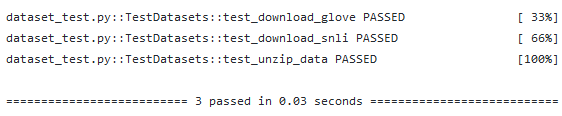
\includegraphics[scale=0.9]{img/dataset_test.png}
                \caption{Test Results for Function 1 Requirements}
                \label{fig:testres1}
            \end{figure}
        
        \subsubsection{Twitter Data Mining Evaluation} \label{twittereval}
            To evaluate the performance of Twitter miner functionality, test cases were used again. This time there are more requirements than in previous subsection, so naturally more test cases are required as well.
            
            The requirements 2.1, 2.2 and 2.7 (see \cref{table:func2spec}) involved connecting to Twitter \gls{api} and fetch new data each time the test is run. For 2.3 - 2.6, a more simple test cases were developed as those requirements deal purely with string manipulation and processing. Overall result is that all cases have passed and requirements are met as expected. \cref{fig:testres2} shows this, as each function name corresponds to a requirement listed in \cref{table:func2spec}.
            
            \begin{figure}[!htbp]
                \centering
                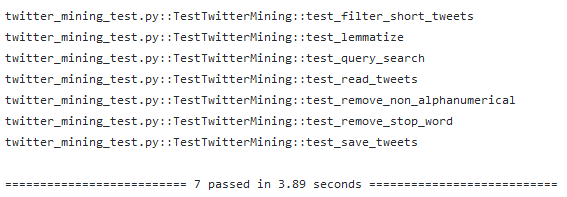
\includegraphics[]{img/twitter_mining_test.png}
                \caption{Test Results for Function 2 Requirements}
                \label{fig:testres2}
            \end{figure}
            
        \subsubsection{LSTM Performance Evaluation} \label{lstmeval}
            The main parameters for evaluating \gls{lstm} performance is accuracy and loss. Accuracy is a percentage value that shows how many samples the model predicted correctly compared to how many there are total. Loss, on the other hand, is not a percentage. It is a summation of the errors made for each example in training, validation and testing sets.
            
            \begin{lstlisting}[language=Python, caption=Accuracy Calculation, label=code:accuracy]
with tf.variable_scope('Accuracy'):
    predicts = tf.cast(tf.argmax(self.__classification_scores, 1), 
                      'int32')
    y_label = tf.cast(tf.argmax(self.__labels, 1), 'int32')
    corrects = tf.equal(predicts, y_label)
    num_corrects = tf.reduce_sum(tf.cast(corrects, tf.float32))
    self.__accuracy = tf.reduce_mean(tf.cast(corrects, tf.float32))
            \end{lstlisting}
            
            The code for evaluating accuracy is presented above (see \cref{code:accuracy}).
            
            \begin{lstlisting}[language=Python, caption=Loss Calculation, label=code:loss]
with tf.variable_scope("loss"):
    cross_entropy = tf.nn.softmax_cross_entropy_with_logits_v2(
          logits=self.__classification_scores, labels=self.__labels)
    self.__loss = tf.reduce_mean(cross_entropy)
    self.__total_loss = self.__loss + self.__weight_decay * 
          tf.add_n(tf.get_collection(tf.GraphKeys.REGULARIZATION_LOSSES))
            \end{lstlisting}
            
            Both Loss and Accuracy calculations involve dynamic variables that are adjusted as needed while the model learns and tries to maximise accuracy and reduce losses. After set amount of steps, the system prints on screen current accuracy and loss values, showing in which direction it is adapting, and whether the values are satisfactory at any given step (see \cref{code:print1}).
            
            \begin{lstlisting}[language=Python, caption=Accuracy and Loss Reporting, label=code:print1]
acc = self.__sess.run(self.__accuracy, feed_dict={self.__hyp: hyps,
                                                self.__evi: evis,
                                                self.__labels: labels,
                                                self.__input_keep: 0.1})
tmp_loss = self.__sess.run(self.__loss, feed_dict={self.__hyp: hyps,
                                                self.__evi: evis,
                                                self.__labels: labels,
                                                self.__input_keep: 0.1})
            \end{lstlisting}
            
            This process is performed during training, validation and testing cycles. Additionally, at the end of each stage (e.g. training), the overall average accuracy and loss values are calculated and printed to the user (code is not shown here in \cref{code:print1}).
            
            If the model results are satisfactory, the model is saved for future use as per software implementation details in previous chapter.
            
            Moving on to requirements, only 3.5 (see \cref{table:func3spec}) was tested using Python unit tests. This is because other requirements (3.1 - 3.4 and 3.6 - 3.8) are hard to test without investing a lot of hardware resources. Figure below shows the results of 3.5 requirement's test:
            
            \begin{figure}[!htbp]
                \centering
                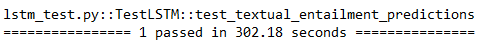
\includegraphics[]{img/test_lstm_entailment.png}
                \caption{Test Results for 3.5 Requirement}
                \label{fig:testres3}
            \end{figure}
            \FloatBarrier
            
            The long execution time is the effect of having to setup the \gls{lstm} from saved model and to run it.
            
            As for the other requirements, to ensure that the system is fully operational, extensive logging is performed, and such logs can be seen in \cref{apx_B}. The logging is set up so that before and after every major action the system outputs its' current state, along with a timestamp.
            
            From the output logs it can be seen that the requirements 3.1 - 3.4 are fulfilled sequentially, one after another. The developed model performs with 78.13\% accuracy, which is above the 75\% margin specified in requirement 3.6. As for saving, it is performed only when training finishes. Loading, on the other hand, is run when the intent is to run the trained \gls{lstm} on twitter data. This requirement can be seen in action in \cref{apx_C}.
            
            \subsubsection{LSTM Trained Accuracy Review} \label{similarworkcompare}
                Since \gls{lstm} is a huge component and one of the core functionalities of the software, it is important to compare its' performance to other, similar existing works and critically evaluate.
                
                \begin{figure}[!htbp]
                    \centering
                    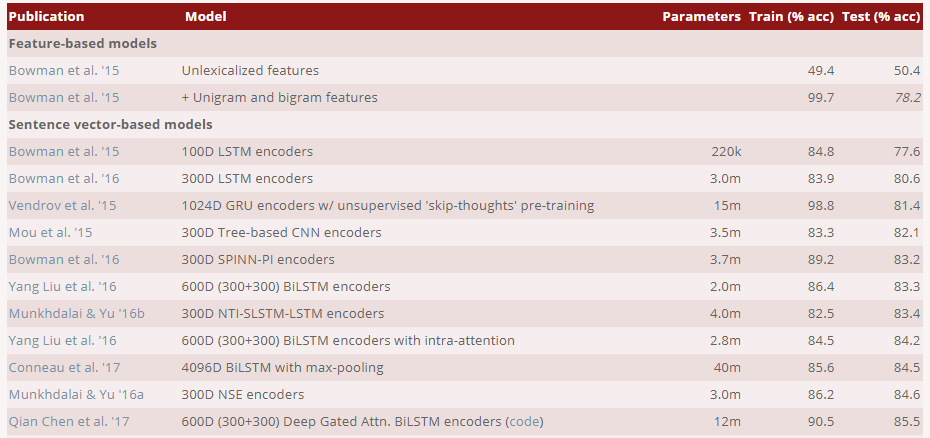
\includegraphics[scale=0.6]{img/snli.png}
                    \caption{A Perspective of Similar Work Performances}
                    \label{fig:snli}
                \end{figure}
                \FloatBarrier
                
                Figure above lists similar work results of recent years, sorted from oldest to newest \autocite{table:snli}. This project falls into the Sentence vector-based models category, so these works are against which the project's performance is going to be compared. As mentioned before, the \gls{lstm} developed here achieves a testing accuracy of 78.13\% which is only slightly above the \textit{100D LSTM encoders} model.
                
                First of all, a bit of context. The numbers with a \textit{D} at the end denote the vector size of the model. These vectors take a lot of \gls{ram} to store them in memory. On top of that, as vector size scales, so do other parameters need to be scaled up, such as the size of \gls{lstm}, for example.
                
                This project uses a vector size of \textit{200D}, which when combined with other \gls{lstm} parameters and the need to store \gls{snli} data in memory for processing, it completely uses up the 16.0 GB of \gls{ram} that the development environment computer has.
                
                When looking at other models that are performing with more accurate results, it is no surprise that they use higher vector sizes, sometimes even multiple vectors or additional components that go hand in hand with \gls{lstm} networks.
                
                In conclusion, it can be said that the model's accuracy is in line with what can and should be expected. On the other hand, it is clear that there is a long way to go to reach super accurate prediction models and even further to be able to run them on home computer conditions for everyday use, such as catching up with social media discussions and online news debates.
            
        \subsubsection{Graph Construction Evaluation} \label{grapheval}
            This section ensures that the functionality of building a graph is working as expected. Among other things, this includes making sure that nodes are created, edges are drawn and differentiated between attack and support and so on.
            
            \begin{figure}[!htbp]
                \centering
                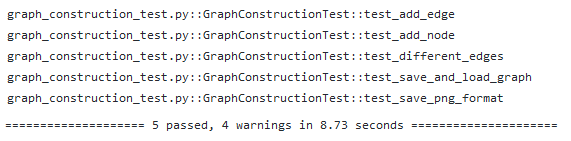
\includegraphics[scale=0.9]{img/graph_construction_test.png}
                \caption{Test Results for Function 4 Requirements}
                \label{fig:testres4}
            \end{figure}
            \FloatBarrier
            
            All of the test cases involve creating a custom graph, which contributed to a higher test running time (8.9 seconds). Requirements 4.1 - 4.3 and 4.7 are tested by simply creating a graph and then assessing if correct nodes, edges or colors are assigned.
            
            For 4.4, 4.5 and 4.8 requirements, the tests are similar in nature to those in \cref{dataeval}. Saved files and their formats are checked by making sure that they exist in the required folder. The loading functionality, however, requires a bit more work to evaluate. First, the graph has to be created and saved, then the graph in memory is set to \textit{null}, or in Python terms, \textit{None}. When the graph is loaded back in, it is evaluated if the same properties remain true that were set during the initial graph creation.
            
            Requirement 4.6 can be tested by simply running the program or any test case that has custom graph in it, can be seen here in \cref{fig:displaygraph} below.
            
            \begin{figure}[!htbp]
                \centering
                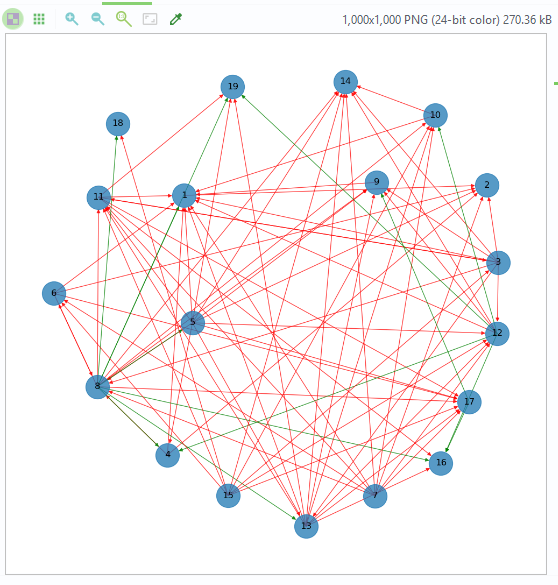
\includegraphics[scale=0.6]{img/display_argument_framework.png}
                \caption{Argument Framework Display}
                \label{fig:displaygraph}
            \end{figure}
            \FloatBarrier
            
            The last requirement, 4.9 is inspected by going into file properties of the image, and checking its' dimensions.
            
            \begin{figure}[!htbp]
                \centering
                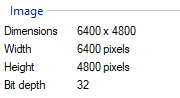
\includegraphics[]{img/high_definition_image_req.png}
                \caption{High Definition Image Dimensions}
                \label{fig:highdef}
            \end{figure}
            \FloatBarrier
            
        \subsubsection{Argument Framework Evaluation} \label{afeval}
            \gls{af} testing requires the creation of a \textit{dummy} \gls{af}, consisting of 4-6 nodes and different relations between them. It is essential to keep the test cases simple and to the point. The requirements 5.1 - 5.3 are tested by assessing the computed conflict free arguments, admissible sets and grounded extension against provided, expected values.
            
            \begin{figure}[!htbp]
                \centering
                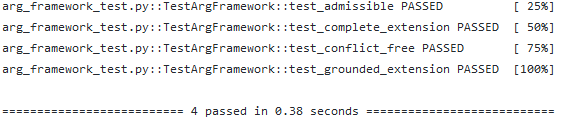
\includegraphics[scale=0.9]{img/arg_framework_test.png}
                \caption{Test Results for Function 5 Requirements}
                \label{fig:testres5}
            \end{figure}
            \FloatBarrier
            
            The remaining requirements, 5.4 - 5.6 are fulfilled as shown in the output log, in \cref{apx_B}.
            
    \subsection{Analysis of Data Mined Argument Frameworks} \label{analysis}
        This section performs an analysis on results generated using this project's software. The main idea here is to analyse what the consensus is with regards to a given topic. The topic will be used as a search term inside Twitter, and the first, most recent tweets will be recorded and argument framework generated out of them.
        
        \subsubsection{Search Term: `Democrats' and `Republicans' Analysis} \label{usaanalysis}
            For this analysis, search terms \textit{Democrats} and \textit{Republicans} were chosen, because those are the two main parties of US government, and intuitively should generate opposing results and view points.
            
            The first argument framework graph is for the search term \textit{Democrats}.
            \begin{figure}[!ht]
                \centering
                \includegraphics[scale=0.3]{img/democrats.png}
                \caption{Argument Framework for `Democrats'}
                \label{fig:demnocrat}
            \end{figure}
            \FloatBarrier
            
            The grounded extension is listed below, including the original, unmodified version of tweets:
            
            \begin{itemize}
                \item Node 7: `@LindseyGrahamSC is absolutely correct  When Democrats talk about needing to ``heal'' the Supreme Court, they mean making it more liberal by any means necessary  It's literal court packing, which should scare every American'
                \item Node 15: `Donald Trump Leads Top Democrats in North Carolina Poll'
                \item Node 18: `@BernieSanders I believe you are describing yourself and other Democrats in Congress who make \$174K per year, yet somehow have accumulated wealth worth \$millions and live in mansions'
            \end{itemize}
            
            Before going any further, same algorithm is run on the term \textit{Republicans}. Here are the results:
            
            \begin{figure}[!htbp]
                \centering
                \includegraphics[scale=0.3]{img/republicans.png}
                \caption{Argument Framework for `Republicans'}
                \label{fig:republican}
            \end{figure}
            \FloatBarrier
            
            And the grounded extension:
            \begin{itemize}
                \item Node 7: `@wiscyfan @TonyBrunoShow @PhillyMayor Most Democrats are corporatists just like Republicans'
                \item Node 8: `@maddow Were the group of Republicans who met w Russians on July 4th from the states Russia asked if interested in investment per your story tonight? Curious, I live in Alabama and Richard Shelby was there'
                \item Node 9: `I’m going to give you a 30 year lesson. Democrats fix the economy, Republicans fuck it up. Stop being fooled by a racist liar. 2020 we have a lot of work to do \#TrumpRecession'
                \item Node 11: `@realNHperson You took the fun out of funny Maybe focus on issues of Republicans rather than latest Democrat obfuscation'
                \item Node 12:` @JohnCornyn Americans don't trust a president that has lied to them over 12,000 times or the Republicans that refuse to hold the corrupt administration accountable because they are profiting off it'
                \item Node 16: `@LindseyGrahamSC When you DON’T HEAR REPUBLICANS SAYING, or DOING ANYTHING to HELP OUR COUNTRY???? but CHOOSE A LYING, CHEATING, THIEF, RAPIST, RACIST, CHILD TRAFFICKER, PEDOPHILIA, ILLITERATE BOY, then WE THE PEOPLE will do EVERYTHING in OUR POWER to MAKE SURE WE DROWN THE COWARDS IN 2020???'
            \end{itemize}
            
            Looking at the graphs, the red arrows represent attacks on arguments and green represent support relations. The large majority of relations are attacks, which is interesting because it implies that due to politics being a controversial subject, people usually express their opinions when they disagree with some points, or are in discontent. On top of that, politics are very subjective in nature, there is not a silver bullet that can solve current political issues, so there might as well be as many opinions as there are people.
            
            The second interesting thing is the fact that when searching for a specific term, the grounded extension is, in this case, a negative opinion involving that query. Neither \textit{democrats} nor \textit{republicans} contain supportive messages in grounded extension, with \textit{republican} \gls{af} not containing a single green arrow.
        
        \subsubsection{Search Term: `Tory' and `Labour' Analysis} \label{ukanalysis}
            The next analysis brings the focus to UK. Here, the terms \textit{Tory} and \textit{Labour} were chosen, which are the two main political parties in UK. With this, the hope is to, first of all, see how these parties are viewed on social media, as they represent the polar opposite ideologies of political spectrum, and secondly, to see if there are any differences or similarities to the previous analysis with the US.
            
            First of all, \gls{af} for the term \textit{Tory}.
            \begin{figure}[!htbp]
                \centering
                \includegraphics[scale=0.3]{img/tory.png}
                \caption{Argument Framework for `Tory'}
                \label{fig:tory}
            \end{figure}
            \FloatBarrier
            
            Accompanied by grounded extension tweets:
            \begin{itemize}
                \item Node 5: `Sarah Wollaston has changed party twice since been elected as a Tory, on a pro-Brexit platform   She once called for MPs switching parties to face automatic by-elections and now refuses to do so herself   Wondering why the public distrust politicians? Sarah is a perfect example'
                \item Node 6: `@LibDems @ChukaUmunna She supported Leave then switched to Remain in last few weeks of EU referendum  Stood on a GE17 Tory Leave manifesto and promised not to back a 2nd referendum  She then backed a 2nd referendum  Sponsored a Bill in HOC for compulsory by-elections for defectors then  defected'
                \item Node 9: `Poverty is no longer a hated symptom, it is a carefully crafted Tory weapon \#dwp \#poverty \#homelessness \#homeless \#OAPs \#PMQs \#pensions \#politics \#parliament \#brexit \#esa \#pips \#wca'
            \end{itemize}
            
            Next, \gls{af} for \textit{Labour}.
            
            \begin{figure}[!htbp]
                \centering
                \includegraphics[scale=0.3]{img/labour.png}
                \caption{Argument Framework for `Labour'}
                \label{fig:labour}
            \end{figure}
            \FloatBarrier
            
            And the grounded extension tweets:
            \begin{itemize}
                \item Node 4: `Jeremy Corbyn has checkmated Jo Swinson \& exposed the Lib Dems again for the vindictive charlatans they are  They've bleated for the last 3 years they want to stop Brexit, they want another vote, but when given the chance by Labour they refuse \#ReachOverTheNoise \#YellowTories'
                \item Node 7: `@GeorgeAylett Ah Labour inflexibility on full show again, combined with its usual effort to blame no deal on everyone else   Nothing to do with the fact that 114 Labour MPs abstained on JC’s orders on the Cherry a Revoke backstop on 1/4/2019    It lost by 112   No deal IS down to LP \& JC''
                \item Node 8: `Sorry, David; I am normally with you on whatever you write   But not with this   You don't seem to understand just how reviled Jeremy Corbyn is!  The man has to be deposed   He has to be got rid of   The Labour Party will only be able to look itself in the mirror afterwards'
                \item Node 14: `@dhothersall No one has yet defined ``brief'' Once in power Labour may move the goalposts - see indyref2 as an example!'
                \item Node 17: `You have been silent for 9 years that @Conservatives have subjected British families to poverty  @UKLabour have tabled a process to block no-deal Brexit while @Conservatives want to shut down Parliament to impose a no-deal  And you still blame Labour, this is perverse'
                \item Node 18: `Agree  and labour are even worse  So we are just country led by Cardiff centric Cartel'
                \item Node 19: `@FaultFinderUK Legal challenge still ongoing (due to Labour's proven use of vote-riggers)  But your bio states that you ``bark at racists'' I suggest you trot on over to Finsbury Park, to the home of your Jew-hating comrade leader currently under investigation for exactly that  There's a good boy'
            \end{itemize}
            
            When comparing the two graphs, it is instantly noticeable that the \gls{af} for \textit{Tory} has quite a few support relations, compared to \textit{Labour}, which has none. A conclusion could be made here that the \textit{Tory} party in the UK, compared to \textit{Labour}, is, at the current political climate, less controversial. Coincidentally, though this is just speculation, it might suggest that people are more in favour of brexit than the news outlets might suggest, because \textit{Tory} party does position itself in favour of leaving the EU.
            
            The \textit{Labour} \gls{af}, on the other hand, not all arguments are specifically against the party. For example, Node 17 from above is clearly arguing for \textit{Labour}. But still, it is undeniable that based on this grounded extension, the opposition party looks to be a lot more controversial.
            
            To contrast this with the US analysis, there are some interesting differences in how the social media treats similar two party government systems. In USA, the discussion involves mainly about the political parties as a whole, with the President's name being mentioned once in a while. UK, on the other hand, has \textit{Party Leaders}. The discussion in UK involves talking about specific actions or stances taken by those individuals who are the faces of the party. It is hard to say why this difference is so stark, but it is interesting nonetheless.

    \subsection{A Review of Project Objectives and Achievements} \label{softachieve}
        This subsection gives an overview of what objectives and aims are achieved at this point. The goal here is to reinforce the reader with concrete examples of accomplishments, specifically with regards to project objectives stated in the beginning. In \cref{aims:objectives}, ten total bullet points were listed, each constituting a project's aim. Here, all bullet points will be referenced to emphasise current achievements.
        
        The first three objectives are to provide an introduction, give technical background on the subject and review existing literature, respectively. \cref{argumentation} and \cref{argumentmining} both give introductions to argumentation as a whole and argument mining. The technical background is extensively covered in \cref{techbackground}, while literature review is presented, critically discussed and evaluated in \cref{literature}. At that point, three aims are already met.
        
        The fourth bullet point states the objective to gather Twitter data, specifically tweets, and preprocess it with the help of stop word elimination and lemmatization. Technical requirements to achieve this are listed in \cref{table:func2spec}, and \cref{twittereval} shows that the requirements are fulfilled. This means that the objective has been met.
        
        Next, the fifth bullet point is concerned with implementing a \gls{lstm} neural network alongside training, validation and testing. Corresponding technical requirements are in \cref{table:func2spec}, and \cref{lstmeval} underlines that proper results are achieved. Another project objective can be crossed off as completed.
        
        The sixth objective tasks the project to recognise textual entailment relationships between tweets. This directly correlates to requirement 3.4 in \cref{table:func3spec}. From \cref{lstmeval} can be seen that this is indeed achieved successfully.
        
        Moving on, the seventh objective says that based on arguments and their relations, a graph representation of it needs to be created. Based on the tests performed in \cref{grapheval} in accordance to \cref{table:func4spec} requirements, it can be noted that a graph was indeed constructed and visually displayed on the screen. This makes the completed objectives count go up to seven out of ten.
        
        The following bullet point is eighth. After the graph representation of \gls{af} is created, the goal is to analyse it and compute the grounded extension, which is exactly what the eighth bullet point states. The previous subsection, namely \cref{afeval}, presents the test results and references technical requirements accordingly (see \cref{table:func5spec} for requirements). The tests indicate that this bullet point has also been met.
        
        The ninth bullet point was done in \cref{usaanalysis} and \cref{ukanalysis} in this chapter. The results were intriguing and gave insight into human behaviour, with, probably, additional analysis possible if performed by a qualified psychologist or anthropology researcher. The latter, the evaluation of neural network and critical comparison of competing models, was done in \cref{similarworkcompare}.
        
        The next two chapters, \cref{conclusions} and \cref{futurework} deal with giving overall conclusions of the project and presenting a discussion of possible future work improvements, respectively. As a matter of fact, this is the last objective from the list, and is fulfilled in the aforementioned sections.
    \section{Conclusion} \label{conclusions}
    This section briefly summarises what has been achieved throughout the project. Analysis performed on two government systems used by English speaking countries showcase interesting social tendencies how the public treats and reacts to opposing parties. It is sufficient to say that this is only the tip of the iceberg and there are many different topics that can be explored in the same manner, not only politics as was chosen here.
    
    The contribution to research community is substantial. The trained classifier is in line with expected performance given the circumstances of hardware limitations, and the overall software is a stepping stone to combining argument mining, extraction, relation detection and framework analysis into one coherent process, with high hopes of becoming an advanced system capable of handling multiple models and multiple social media platforms.
    \section{Future Work} \label{futurework}
    While the project is ambitious in its goal to combine argument mining, argument relation detection and argument framework analysis into a single coherent system, it is far from being complete in its current iteration. This chapter considers a multitude of possible improvements that could be implemented to further the quality of the project in future.
    
    First of all, technical bottlenecks should be eliminated. This means that due to the scale of the project, additional hardware resources are required which could potentially free up space for innovation and additional parameter tuning. Currently, the system hinges on a 78\% rate of predictions being accurate, which is great considering the circumstances, but there is a lot of room for improvement.
    
    Secondly, at the moment the user interface is very minimal and requires programming language knowledge from the user to operate it. Eliminating this factor would be ideal to bring the software closer to the user.
    
    The third possible improvement is to completely adopt the micro services architecture. This would mean that the project has to be broken up into distinct components and hosted on the cloud. What this does is allows for future collaboration, where each component acts as a plugin, that can be easily added or removed based on user's needs and goals. For example, a user might first want to train a model or use an existing one to simply perform argument framework analysis, or, alternatively, train the model and in the same cycle test it on live data for comparison. Additionally, it would be possible to develop and easily integrate a whole different model, that does not use \gls{lstm} at all, and is something completely new and innovative. On the other hand, other existing models that are developed by others should not be ignored and could be incorporated into the project alongside existing implementation. For example, back in \cref{deeplearning}, one similar approach was mentioned, that reached 89.53\% accuracy rate, improving which could be seen as the next milestone for the project.
    
    Next, the software is currently limited to Twitter. While Twitter is a popular social media platform, it is not the only one, and so it could be expanded to support other platforms, which would enable the system to perform analysis on a much more wider scale.
    
    Last but not least, the software can be rebuilt from the ground up using custom made solutions. While this is a time expensive option, there are some benefits to this. One is that the programming language can be chosen based on needs, not the availability of certain specific libraries. Secondly, most libraries are developed to be general purpose, available for use to most problems. In this domain, it might be preferable to build and tune the library functions specifically to argument mining, given that this is a pretty young research field.
    
    In conclusion, there are many pathways the project can be taken from this point onwards. While not all approaches are must-haves, the important fact is that there are limitless possibilities to how the project can be shaped to be in the future, and all of them are promising in their own way.
    
    
    
    \printbibliography
    %\thispagestyle{empty}


\mbox{}\newline\vspace{10mm} \mbox{}\LARGE
%
{\bf Declaration} \normalsize \vspace{5mm}

I declare that this thesis is the solely effort of the author.
I did not use any other sources and references than the listed ones. I have marked all contained direct or indirect statements from other sources as such.

Neither this work nor significant parts of it were part of another review process.
I did not publish this work partially or completely yet.
The electronic copy is consistent with all submitted copies.

\bigskip
\bigskip
\bigskip
\bigskip


Signature and date: 





    \appendix
    \section{Schedule and Planning} \label{apx_A}
    \begin{table}[!htbp]
    \centering
    \begin{tabular}{|l|c|c|c|c|c|c|c|c|c|c|c|c|c|c|c|c|}
        \toprule
        & \multicolumn{4}{c|}{May} & \multicolumn{4}{c|}{June} & \multicolumn{4}{c|}{July} & \multicolumn{4}{c|}{August} \\ 
        \midrule
        
        Research Code Libraries & \multicolumn{2}{c|}{\cellcolor{brown}} & & & & & & & & & & & & & & \\
        \hline
        Web Scraper Implementation & & & \multicolumn{2}{c|}{\cellcolor{blue}} & & & & & & & & & & & & \\
        \hline
        
        Social Media Data Mining & & & & & \multicolumn{3}{c|}{\cellcolor{orange}} & & & & & & & & & \\
        \hline
        
        Implementation of \gls{te} Algorithms & & & & & & & & \multicolumn{2}{c|}{\cellcolor{green}} & & & & & & & \\
        \hline
        
        Evaluation of \gls{te} Algorithms & & & & & & & & & & \cellcolor{red} & & & & & & \\
        \hline
        
        Implementation of \gls{af} & & & & & & & & & & & \multicolumn{2}{c|}{\cellcolor{gray}} & & & & \\
        \hline
        
        Overall System Testing & & & & & & & & & & & & & \cellcolor{yellow} & & & \\
        \hline
        
        Conclusion, Presentation, Future Work & & & & & & & & & & & & & & \multicolumn{2}{c|}{\cellcolor{purple}} & \\
        \bottomrule
    \end{tabular}
    \caption{Proposed timetable for MSc Individual Project}
    \label{table:timetable}
\end{table}
    
    Short description of each goal:
    \begin{itemize}
        \item Research Code Libraries - analysing existing code libraries and frameworks, making a choice on programming language, etc.
        \item Web Scraper - decide on a mechanism of extracting text/arguments from social media, whether that's a manually coded web scraper or access to \gls{api} if there is one.
        \item Social Media Data Mining - transforming raw text into data structures for future \gls{te} algorithm use.
        \item Implementation of \gls{te} Algorithms - implementing the \gls{te} algorithm with specific properties/parameters that suit the project.
        \item Evaluation of \gls{te} Algorithms - testing and evaluating the results of the algorithms implemented.
        \item Implementation of \gls{af} - using the results of \gls{te} algorithm to build \gls{af}.
        \item Overall System Testing - putting everything together into a coherent project and performing overall evaluation.
        \item Conclusion, Presentation, Future Work - drawing appropriate conclusions of the project, proposing future work areas or possible improvements, creating presentation slides, other finishing works.
    \end{itemize}

    \section{Model Training Output Log} \label{apx_B}
    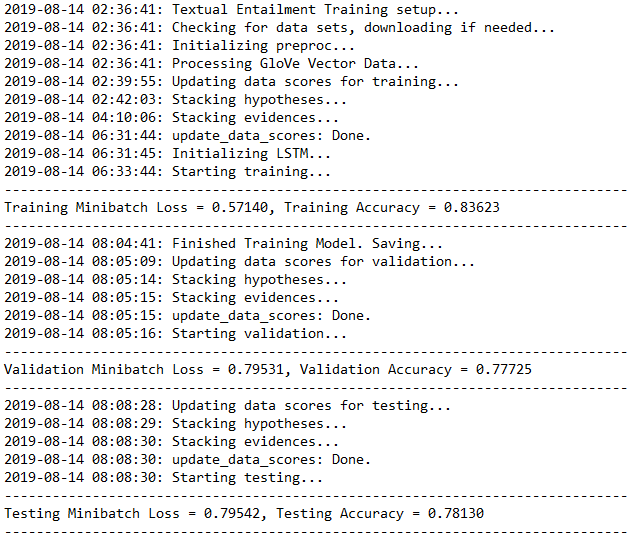
\includegraphics[]{img/training_log.png}
    \section{Application Output Log} \label{apx_C}
    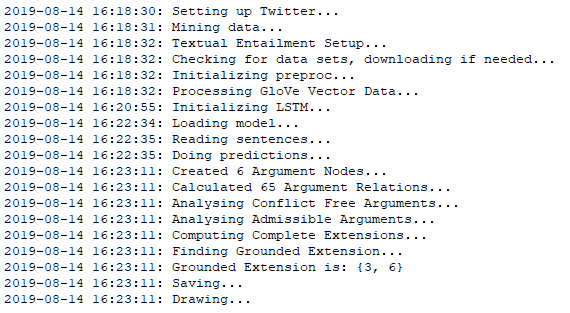
\includegraphics[]{img/application_log.png}

\end{document}
